\documentclass[conference]{IEEEtran}
\IEEEoverridecommandlockouts
\usepackage{amsmath,amssymb,amsthm}
\usepackage{graphicx}
\usepackage{booktabs}
\usepackage{url}
\usepackage{xcolor}
\usepackage{enumitem}
\setlist{nosep,leftmargin=*,itemsep=1pt}
\newtheorem{proposition}{Proposition}
\emergencystretch=2em
\renewcommand{\topfraction}{0.95}\renewcommand{\bottomfraction}{0.8}\renewcommand{\textfraction}{0.05}\renewcommand{\floatpagefraction}{0.8}
\renewcommand{\dbltopfraction}{0.95}\renewcommand{\dblfloatpagefraction}{0.8}
\setcounter{topnumber}{3}\setcounter{dbltopnumber}{3}\setcounter{totalnumber}{6}
\begin{document}
\title{Is It the Beliefs? A Matched-Information Study of Hidden-Rule Discovery by Hypothesis-Testing, Bayesian and Learned Agents}
\author{\IEEEauthorblockN{Mihit Nanda$^{*}$}
\IEEEauthorblockA{IILM University\\
Greater Noida, India}
\and
\IEEEauthorblockN{Sanju Tiwari}
\IEEEauthorblockA{Sharda University\\
Greater Noida, India}}
\maketitle

\begin{abstract}
Hidden-rule discovery asks an agent to infer, from the consequences of its own actions, rules it was never told. Recent discovery benchmarks target language-model agents and report end-to-end success, which leaves open \emph{why} explicit hypothesis testing outperforms learned policies: the architecture, or the belief information it maintains? We answer with a matched-information design. A hypothesis-testing agent, posterior sampling and PPO agents act over one macro-action vocabulary in a procedural grid world (six generalization regimes), a combination vault and a noisy variant, and one learned agent also receives the tracker's beliefs as input. The hypothesis agent's advantage splits exactly into an information gap and a learning gap, estimated over independently trained models. At difficulty 5, learned agents without beliefs reach 55\% against 74\%; adding beliefs recovers 74\%, so almost all of the gap is information (0.19) and the remaining learning gap is indistinguishable from zero (-0.001). The same pattern holds for unseen color symbols (0.64, 0.98 with beliefs, 0.98 for the tracker). A hard exclusivity assumption fails when false (0.23 success); a soft prior restores 1.00. On the survival part of CausalGame, where no hypothesis space is supplied, an expected-value-plus-information-gain agent does not beat random search. The environments are synthetic and the vocabularies hand-built.
\end{abstract}
\begin{IEEEkeywords}
rule discovery, hypothesis testing, matched-information control, posterior sampling, meta-reinforcement learning
\end{IEEEkeywords}

\section{Introduction}
Agents in new environments are rarely told the rules. They must infer which key opens which door, or which lever order opens a vault, from the consequences of their own actions. Recent work probes this ability in language-model agents on interactive discovery benchmarks~\cite{jansen2024,gandhi2025,chen2026causalgame} and abstract-reasoning suites~\cite{chollet2025arc2}, and studies hypothesis generation and in-context exploration in such models~\cite{wang2024hs,krishnamurthy2024}. In reinforcement learning (RL), theory-based agents~\cite{tsividis2021} and large memory-based meta-RL agents~\cite{ada2023} both adapt quickly, and recurrent model-free RL is a strong baseline for partially observable problems when implemented with care~\cite{ni2022}. These lines do not separate \emph{why} explicit hypothesis testing so often wins in small controlled settings: is it the architecture, or the belief information it carries (a hypothesis space, a memory of outcomes, and the exclusion of refuted hypotheses)? The answer decides whether beliefs should be built into agents or can be expected to be learned.

We study the question in fully inspectable environments with a \emph{matched-information control}: a learned agent that is given the hypothesis tracker's beliefs as input and is otherwise unchanged. Our contributions are:
\begin{itemize}
\item a matched-information design with an exact decomposition of the hypothesis agent's advantage into an \emph{information gap} and a \emph{learning gap} (Sect.~\ref{sec:belief});
\item a controlled comparison over a shared macro-action vocabulary in a grid benchmark with six generalization regimes and a combination vault, with statistics over independently trained models (15 for the main learned agents, fewer elsewhere; 65 pre-declared comparisons, Holm-corrected);
\item robustness tests: a false structural assumption and a soft prior that repairs it for detectable violations, jammed-lock noise, and a non-language check on the survival part of CausalGame~\cite{chen2026causalgame};
\item an elementary failure-cost proposition used as an analytical check, and code, data and models at \url{https://github.com/mihiit/RuleDiscovery}.
\end{itemize}
The comparison is deliberately asymmetric in what agents know, so every gap is conditional on the structure supplied (Table~\ref{tab:info}); no claim is made about general intelligence, ARC-AGI-style tasks or real-world discovery.

\section{Related Work}
\textbf{Discovery benchmarks (2024--2026).} DiscoveryWorld~\cite{jansen2024} offers 24 simulated scientific tasks on which strong baseline language agents struggle. BoxingGym~\cite{gandhi2025} scores experimental design by expected information gain and reports that adding an explicit statistical model did not reliably help its LLM agents. CausalGame~\cite{chen2026causalgame} places an LLM agent in a drone-design game with hidden confounders and selection bias. ARC-AGI-2~\cite{chollet2025arc2} tests few-shot abstraction on static grids. All evaluate language agents end to end; none of them, to our knowledge, varies only the belief information given to a learned non-language agent over a fixed action vocabulary.

\textbf{Hypotheses and adaptation.} Theory-based RL learns program-like game models by Bayesian inference and matches human learning efficiency~\cite{tsividis2021}; Hypothesis Search has an LLM propose and test explicit hypotheses~\cite{wang2024hs}. LLM exploration improves when the interaction history is externally summarized as sufficient statistics~\cite{krishnamurthy2024}, which parallels our belief inputs. Large meta-RL agents show hypothesis-driven exploration when trained over vast task distributions~\cite{ada2023}; RL$^2$ and variBAD are the classical recurrent and Bayes-adaptive baselines~\cite{duan2016,zintgraf2020}, and recurrent model-free RL needs careful implementation to be competitive~\cite{ni2022}. Posterior sampling~\cite{strens2000,osband2013} and information-directed exploration~\cite{russo2014} give our Bayesian baseline and our utility.

\textbf{Evaluation.} Generalization surveys and benchmarks~\cite{kirk2023,chevalier2023,cobbe2020} motivate our held-out regimes, and guidance on RL statistics~\cite{agarwal2021,patterson2024} motivates treating the trained model, not the evaluation episode, as the unit of replication.

\textbf{Positioning.} Hypothesis testing, posterior sampling and information gain are established. Our contribution is empirical: the matched control and its decomposition, training-run-level statistics, and robustness tests, in a setting small enough to be fully inspected. Prior comparisons often change the action space, the evidence kept and the evaluation protocol at once; here only the belief input is varied.

\section{Method}
\subsection{Belief view and decomposition}\label{sec:belief}
Let $\theta$ be the hidden rule table (key--door, switch--bridge, push-block bindings), $h_t$ the history of actions and outcomes, and $b_t=P(\theta\mid h_t)$ the belief. The task is a partially observable decision problem whose only unobserved component is $\theta$~\cite{kaelbling1998}.
\begin{proposition}[Belief sufficiency; classical]\label{prop:suff}
For any history-dependent policy there is a policy that depends on $h_t$ only through $(o_t,b_t)$ and attains the same value; in particular an optimal policy exists of this form.
\end{proposition}
A policy without $b_t$ must carry an equivalent summary in its recurrent state; one given $b_t$ need only learn the map from beliefs to actions. Our tracker supplies an \emph{approximate} $\hat b_t$ (confidences with exclusion of refuted hypotheses, not an exact posterior), so Proposition~\ref{prop:suff} motivates the design but gives no guarantee. Writing $S_H$, $S_L$ and $S_{L+b}$ for the success of the tracker agent, a learned agent, and the learned agent given $\hat b_t$, the advantage decomposes exactly:
\begin{equation}
S_H-S_L=\underbrace{(S_{L+b}-S_L)}_{\text{information gap}}+\underbrace{(S_H-S_{L+b})}_{\text{learning gap}}.\label{eq:dec}
\end{equation}
The matched control estimates the first term; the second is what remains for the policy to learn.

\subsection{Environments}
\textbf{Grid.} Fully observable $8$--$14$-cell grids with walls, keys, doors, switches, chasms, movable blocks, traps and a target; rules are composed from key--door (one key carried at a time; key color $k$ opens door $\phi(k)$), switch--bridge and push-block gates, and are never observed. Difficulty 1--5 adds gates, distractors and traps; an episode lasts at most 200 steps, and every instance is solvable by construction. Regimes: A (train single rules, test pairs), B (pairs to the triple), C (longer chains, $12{\times}12$), C2 (same rules, $14{\times}14$), D (four unseen color symbols, same key-equals-door relation) and E (train KD and SB+PB, test the triple).

\textbf{Vault.} A hidden injective sequence of $k$ of $L$ levers must be pressed in order; a wrong press resets progress. Learned agents train on $L\in\{4,5\}$, $k\in\{2,3\}$ and are tested also on $L\in\{6,7\}$, $k\in\{4,5\}$.

\textbf{Noise and external check.} In the noisy grid a correct key jams with probability $\epsilon$ (same feedback as a wrong key). For CausalGame we drive its released simulator (14 scenarios) with non-language agents on its own budget (10 deployments of 20 drones, then one design scored on 1{,}000 drones), evaluating survival only.

\subsection{Agents}
\begin{table*}[!t]
\caption{Information each agent is given. ``Templates'': hand-built hypothesis forms; $n$: independently trained models (main distribution).}\label{tab:info}
\centering\footnotesize
\begin{tabular}{llllll}
\toprule
Agent & Actions & Evidence kept & Templates & Exclusivity & $n$ \\
\midrule
Reactive & primitives & lose-shift bit & no & -- & -- \\
PSRL & macros & outcome log & yes & hard & -- \\
Hypothesis (tracker) & macros & log, confidences & yes & hard & -- \\
Hypothesis-adaptive & macros & log, confidences & yes & soft prior & -- \\
Macro-FF / GRU & macros & last outcome (+GRU state) & implicit & implicit & 15 \\
Macro-GRU+belief & macros & tracker beliefs as inputs & via tracker & via tracker & 15 \\
Generic-FF / GRU & generic skills & last outcome (+GRU state) & implicit & implicit & 2 \\
Primitive PPO & primitives & GRU state & implicit & implicit & 1 \\
\bottomrule
\end{tabular}
\end{table*}

All agents know the action semantics and avoid traps. The \emph{tracker} keeps a confidence per candidate binding (+0.6 for a correct prediction, $-0.6$ for a wrong one, rejection after two contradictions), recomputes its state from episodic memory, excludes a key already confirmed for one door from others (\emph{exclusivity}), and scores macro-actions by
\begin{equation}
U(a)=V\,p-\mu\,c(a)+\lambda\,H_b(p),\label{eq:u}
\end{equation}
with $p$ the probability the tested hypothesis is true, $c$ the path length, $V=3$ per gate (10 for the target), $\mu=0.05$ and $\lambda=0.5$ (hand-set). \emph{PSRL}~\cite{strens2000,osband2013} keeps one sampled binding consistent with all outcomes and acts as if it were true. The \emph{adaptive} tracker replaces hard exclusivity by a prior: a confirmed key keeps weight $\rho=0.05$ for other doors and the prior is dropped once one key is confirmed for two doors. Learned agents use PPO~\cite{schulman2017} in JAX~\cite{jax2018}, feedforward or GRU~\cite{cho2014}. \emph{Macro} agents choose among the same macro-actions with features limited to macro type, colors, path cost and the last outcome. \emph{Macro-GRU+belief} adds the tracker's $R=Vp$ and $H_b(p)$ per candidate. \emph{Generic} agents choose among go-to-object skills only; \emph{primitive} PPO acts on a CNN encoding of the grid.

\subsection{Protocol and statistics}
Every cell uses 30 evaluation seeds of 30 environments. For agents without trained weights the unit is the evaluation seed; for a learned agent it is the \emph{trained model} (seed $s$ uses model $s \bmod m$). Intervals are 95\% percentile bootstraps over units; tests are Welch's $t$ on unit scores with Holm correction~\cite{holm1979} over the 65 pre-declared comparisons; effect sizes are Cohen's $d$. Where an agent never fails we also give the rule-of-three bound $3/N$.
\begin{proposition}[Failed-test cost]\label{prop:cost}
For one door with $n$ equally likely keys, an agent that never retests a failed key makes $(n-1)/2$ failed tests in expectation; a stateless lose-shift agent makes $(n-1)^2/n$, an excess of $(n-1)(n-2)/(2n)$. In the vault, elimination makes $\sum_{p=0}^{k-1}(L-p-1)/2$ resets in expectation.
\end{proposition}
\emph{Proof sketch.} Elimination tests keys in a uniform random order, so failures before success are uniform on $\{0,\dots,n-1\}$. Lose-shift fails first with probability $(n-1)/n$ and then needs a geometric number of draws with success probability $1/(n-1)$, i.e.\ $n-2$ further failures: $\tfrac{n-1}{n}(1+(n-2))$. In the vault, position $p$ has $L-p$ equally likely levers and replaying the known prefix is not a failure. \hfill$\square$

A second elementary point explains the master-key failure: a prior with zero mass on the true hypothesis cannot be corrected by any evidence (Cromwell's rule), so hard exclusivity fails when false, while $\rho>0$ keeps the true binding testable.

\section{Results}
\begin{table*}[!t]
\caption{Success by difficulty and on unseen color symbols (regime D, held out): mean [95\% bootstrap CI over units]. Units: evaluation seeds, or trained models for learned agents ($n$).}\label{tab:main}
\centering\footnotesize
\begin{tabular}{lcccc}
\toprule
Agent & $d=3$ & $d=4$ & $d=5$ & Unseen colors (D) \\
\midrule
Reactive & 0.397 [0.364, 0.429] & 0.080 [0.063, 0.098] & 0.074 [0.054, 0.096] & 0.118 [0.098, 0.138] \\
PSRL & 0.982 [0.973, 0.990] & 0.879 [0.861, 0.896] & 0.656 [0.624, 0.686] & 0.891 [0.876, 0.907] \\
Hypothesis & 0.981 [0.972, 0.989] & 0.930 [0.916, 0.944] & 0.736 [0.714, 0.758] & 0.981 [0.973, 0.988] \\
Hypothesis-adaptive & 0.981 [0.972, 0.989] & 0.930 [0.916, 0.944] & 0.733 [0.712, 0.756] & 0.981 [0.973, 0.988] \\
Macro-FF ($n=15$) & 0.980 [0.969, 0.989] & 0.757 [0.724, 0.789] & 0.570 [0.542, 0.597] & 0.564 [0.522, 0.607] \\
Macro-GRU ($n=15$) & 0.979 [0.968, 0.988] & 0.778 [0.744, 0.812] & 0.550 [0.523, 0.578] & 0.640 [0.584, 0.694] \\
Macro-GRU+belief ($n=15$) & 0.976 [0.964, 0.986] & 0.918 [0.894, 0.941] & 0.737 [0.706, 0.767] & 0.977 [0.967, 0.986] \\
Generic-GRU ($n=2$) & 0.940 [0.929, 0.951] & 0.561 [0.553, 0.569] & 0.352 [0.327, 0.378] & -- \\
PPO-GRU (primitive) ($n=1$) & 0.000 [0.000, 0.000] & 0.000 [0.000, 0.000] & 0.000 [0.000, 0.000] & -- \\
\bottomrule
\end{tabular}
\end{table*}

\subsection{Matched-information control}
Table~\ref{tab:main} and Fig.~\ref{fig:main}a give success by difficulty. At difficulty 3 every macro-level agent solves almost all episodes ($\geq$0.98) against 0.40 for the reactive agent; primitive PPO reaches 0.00 and is under-trained. Differences appear at difficulty 4--5. At difficulty 5 the tracker agent exceeds the plain Macro-GRU ($\Delta=+0.186$ [+0.151, +0.220]), and the belief-augmented agent exceeds it by the same margin ($\Delta=+0.187$ [+0.144, +0.227]) while being indistinguishable from the tracker ($\Delta=-0.001$ [-0.038, +0.037], $p_{\mathrm{Holm}}=1.00$); Table~\ref{tab:res}(b) lists further Holm-corrected comparisons. Table~\ref{tab:res}(a) gives the decomposition of Eq.~\eqref{eq:dec} with intervals. At difficulty 5: total advantage 0.186, information gap 0.187, learning gap -0.001. At difficulty 4 the corresponding values are 0.152, 0.140 and 0.012. PSRL lies between (0.66 at difficulty 5; tracker against PSRL $\Delta=+0.080$ [+0.043, +0.119]).

\emph{What this does and does not show.} The tracker supplies, per candidate, an expected value and an information gain; producing them already requires the templates, memory and exclusivity rule. The network still has to learn how to act on them. Whether a network could derive such beliefs from raw observations is not tested. With 15 belief-agent runs the smallest difference detectable at 80\% power is about 0.06; failing to separate two agents is not evidence that they are equal.

\begin{figure*}[!t]
\centering
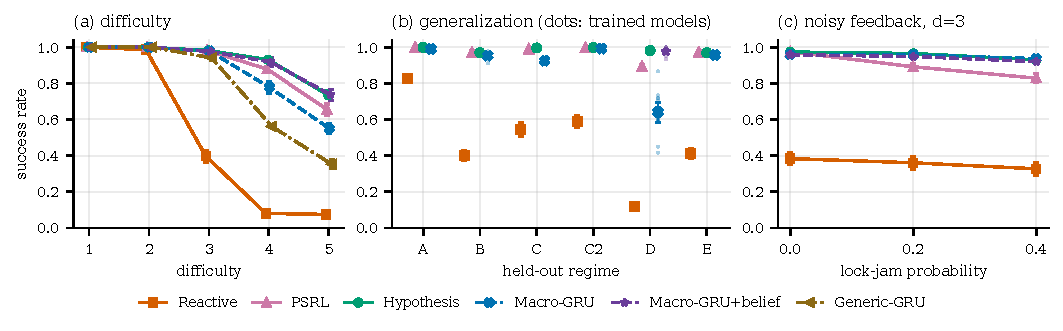
\includegraphics[width=\textwidth]{figures_ieee6/fig6_main.pdf}
\caption{(a) Success by difficulty. (b) Held-out success per regime (regime D: unseen color symbols); dots are individual trained models. (c) Success at difficulty 3 when a correct key jams with the given probability (learned agents trained noise-free). Bars: 95\% bootstrap intervals over units.}\label{fig:main}
\end{figure*}

\subsection{Generalization}
Recombination (A, B, E) and size (C2) are harder for the reactive agent only; longer chains (C) cost the learned agents about 0.08 (Fig.~\ref{fig:main}b). The decisive regime is D: with 15 runs, Macro-GRU scores 0.998 on its training distribution but 0.640 on unseen colors (Macro-FF 0.564), while the tracker is unaffected (0.981). The belief-augmented agent reaches 0.977, indistinguishable from the tracker ($\Delta=+0.004$ [-0.008, +0.017], $p_{\mathrm{Holm}}=1.00$) and far above the plain agent ($\Delta=+0.337$ [+0.283, +0.392]): its inputs do not mention colors, so the failure is one of symbol-specific policies. Regimes B, C, E use 10 runs and A, C2 use 3; those cells are indicative.

\subsection{What matters inside the tracker}
In a reward-form $\times$ information-bonus ablation at difficulty 5, raising $\lambda$ from 0 to 8 lifts success from 0.68 to 0.87 with expected-value reward and from 0.66 to 0.79 with sampled reward (Fig.~\ref{fig:second}d). Memory and revision are necessary (difficulty 4: 0.93 with memory, 0.00 without; 0.93 with revision, 0.23 without); the bonus matters only where distractors make uncertainty costly.

\subsection{False assumptions, noise and the vault}
The tracker's exclusivity assumption is catastrophic when false: when one key opens several doors it succeeds in 0.23 (difficulty 3) and 0.18 (difficulty 4) of episodes, against 1.00 and 1.00 without the assumption, which in turn costs about 0.12 when it is true. The soft prior recovers 1.00 and 1.00 and matches the hard rule on the exclusive control ($\Delta=-0.001$ [-0.016, +0.013], $p_{\mathrm{Holm}}=1.00$); this repairs a \emph{detectable} violation only (Fig.~\ref{fig:second}c). With jammed locks, PSRL drops from 0.97 to 0.83 at $\epsilon=0.4$ and difficulty 3 while the tracker falls from 0.97 to 0.93 ($\Delta=+0.102$ [+0.073, +0.130]); the noise-free-trained learned agents reach 0.94 (Macro-GRU) and 0.92 (with beliefs). At difficulty 4 all agents lose a similar amount, so this is not a general advantage of explicit testing.

In the vault the elimination agent opens every code (1.00, 1.00; 95\% failure-rate bound 0.33\% for 900 episodes) with 3.30 and 8.37 failed presses against 3.33 and 8.32 predicted by Proposition~\ref{prop:cost}; on the grid, single-gate environments give 0.541 failed door tests at difficulty 4 against 0.543 predicted. PPO-GRU solves small codes (1.00) but only 0.14 of larger ones over 10 runs ($\Delta=+0.858$ [+0.837, +0.879]).


\subsection{External check: CausalGame}
On the survival part of CausalGame~\cite{chen2026causalgame} (14 scenarios, 40 sessions per agent and scenario; unit: scenario) every search agent beats the default design (EV+IG against default: $\Delta=+0.046$, $p_{\mathrm{Holm}}=0.003$), but the EV+IG agent, which uses the same Bayesian model as posterior sampling and picks experiments by expected survival plus an information bonus, is not better than the simpler ones (Table~\ref{tab:res}(c)); the bonus makes no detectable difference. No hypothesis space matching the generator is supplied here, which is consistent with Sect.~\ref{sec:belief}: the benefit of explicit hypotheses depends on a hypothesis space that fits the environment. The benchmark's LLM-judged report rubric cannot be applied to these agents, and our numbers are not comparable to its leaderboard.

\begin{table*}[!t]
\caption{Results with intervals. (a) Decomposition of the tracker's advantage over Macro-GRU (Eq.~\eqref{eq:dec}): total $S_H-S_L$, information gap $S_{L+b}-S_L$, learning gap $S_H-S_{L+b}$, as $\Delta$ success [95\% CI over units]; learned agents: 15 trained models (belief agent 15). (b) Key comparisons (first minus second) from the 65 Holm-corrected tests: $\Delta$, 95\% CI, adjusted $p$, Cohen's $d$; all tests are in \texttt{paper/tables/primary\_comparisons.csv}. (c) CausalGame, survival part: mean over 14 scenarios [95\% CI over scenarios]; success = share of sessions reaching the scenario threshold.}\label{tab:res}
\centering\scriptsize\setlength{\tabcolsep}{3pt}
\begin{minipage}[t]{0.57\textwidth}\centering\textbf{(a)}\\[2pt]
\begin{tabular}{lccc}
\toprule
Condition & Total & Information gap & Learning gap \\
\midrule
difficulty 3 & +0.002 [-0.010, +0.016] & -0.003 [-0.018, +0.012] & +0.006 [-0.009, +0.020] \\
difficulty 4 & +0.152 [+0.116, +0.189] & +0.140 [+0.099, +0.181] & +0.012 [-0.016, +0.040] \\
difficulty 5 & +0.186 [+0.151, +0.220] & +0.187 [+0.144, +0.227] & -0.001 [-0.038, +0.037] \\
unseen colors (D) & +0.341 [+0.289, +0.397] & +0.337 [+0.283, +0.392] & +0.004 [-0.008, +0.017] \\
\bottomrule
\end{tabular}\\[6pt]\textbf{(b)}\\[2pt]
\begin{tabular}{lrrrr}
\toprule
Comparison & $\Delta$ & 95\% CI & $p_{\text{Holm}}$ & $d$ \\
\midrule
d5: tracker vs PSRL & +0.080 & [+0.043, +0.119] & 0.01 & 1.0 \\
d5: tracker vs reactive & +0.661 & [+0.631, +0.691] & $<$0.001 & 11.1 \\
master key d3: adaptive vs hard & +0.770 & [+0.737, +0.802] & $<$0.001 & 12.0 \\
master key d4: adaptive vs hard & +0.818 & [+0.791, +0.842] & $<$0.001 & 15.5 \\
control d4: adaptive vs hard & -0.001 & [-0.016, +0.013] & 1.00 & -0.0 \\
D: tracker vs PSRL & +0.090 & [+0.072, +0.107] & $<$0.001 & 2.5 \\
vault larger: tracker vs PPO-GRU & +0.858 & [+0.837, +0.879] & $<$0.001 & 48.2 \\
slip 0.4, d3: tracker vs PSRL & +0.102 & [+0.073, +0.130] & $<$0.001 & 1.8 \\
slip 0.4, d4: tracker vs PSRL & +0.110 & [+0.048, +0.172] & 0.04 & 0.9 \\
\bottomrule
\end{tabular}
\end{minipage}\hfill
\begin{minipage}[t]{0.40\textwidth}\centering\textbf{(c)}\\[2pt]
\begin{tabular}{lcc}
\toprule
Agent & Survival & Success \\
\midrule
Default design & 0.572 [0.489, 0.643] & 0.000 \\
Random search & 0.667 [0.584, 0.724] & 0.398 \\
Hill-climbing & 0.665 [0.587, 0.712] & 0.243 \\
Posterior sampling & 0.637 [0.566, 0.697] & 0.287 \\
EV, no info bonus & 0.623 [0.554, 0.682] & 0.182 \\
EV + info gain & 0.618 [0.542, 0.688] & 0.287 \\
\bottomrule
\end{tabular}
\end{minipage}
\end{table*}


\begin{figure*}[!t]
\centering
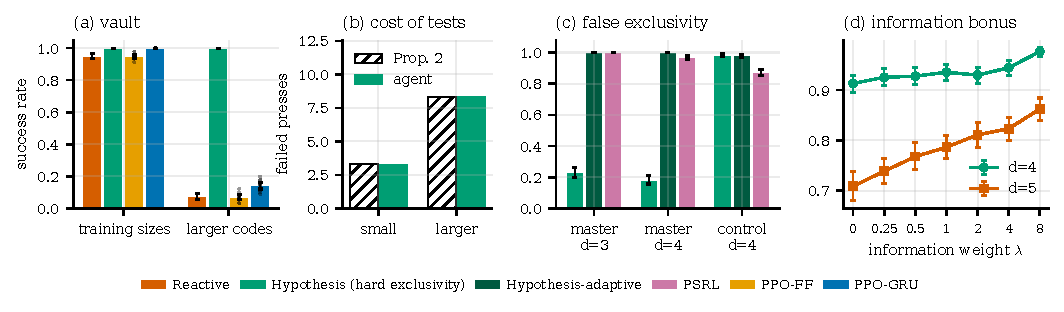
\includegraphics[width=\textwidth]{figures_ieee6/fig6_second.pdf}
\caption{(a) Vault success on training and larger code sizes (dots: trained models). (b) Failed presses of the elimination agent against Proposition~\ref{prop:cost}. (c) One key opens several doors (master) and an exclusive control: hard, adaptive and PSRL agents. (d) Information weight $\lambda$ at difficulties 4 and 5.}\label{fig:second}
\end{figure*}

\section{Discussion and Limitations}
Hypothesis testing helps here chiefly because it keeps a belief state: a learned agent given that state matches it at difficulty 5 and on unseen color symbols, where the supplied features are symbol-free. This agrees with the view that externally maintained sufficient statistics help sequential decision makers~\cite{krishnamurthy2024}, and it narrows the claim: the advantage is largely in what is told to the agent about its own uncertainty. The limitations are real:
\begin{enumerate}
\item \emph{Scale and realism.} Both families are synthetic and, apart from jammed locks, deterministic and fully observable; no real-world data are used.
\item \emph{Hand-built interface.} The templates, macro-actions and generic skills are hand-specified and match the generators.
\item \emph{Baselines.} Primitive PPO is under-trained, and our recurrent agents use on-policy PPO with little tuning; stronger recurrent baselines~\cite{ni2022} and large-scale meta-RL~\cite{ada2023} may narrow the information gap without beliefs.
\item \emph{Training runs.} 15 (main, D), 15 (belief), 10 (B, C, E), 3 (A, C2), 2 (generic, no inference) and one (primitive) models.
\item \emph{Finite samples and constants.} Perfect scores say nothing beyond their samples; $V,\mu,\alpha,\beta,\lambda,\rho$ were set by hand.
\item \emph{External check.} CausalGame covers survival only, with generic surrogate searchers; language agents are not studied.
\end{enumerate}

\section{Conclusion}
In a controlled setting, the advantage of an explicit hypothesis tracker over learned agents is largely an information gap: a learned agent given the tracker's beliefs matches it at the hardest difficulty and on unseen color symbols, with a residual learning gap not distinguishable from zero, and the plain agent does not. A hard exclusivity assumption is catastrophic when false and a soft prior repairs detectable violations; under jammed locks PSRL degrades at difficulty 3; and on CausalGame, where no hypothesis space is supplied, the information-gain agent does not beat simple search. These are results for synthetic, mostly deterministic benchmarks with hand-built interfaces. Open questions are whether belief features can be learned from raw observations and whether the findings survive partial observability and language agents.

\section*{Reproducibility Statement}
The source code is available at : \url{https://github.com/mihiit/RuleDiscovery}

\textbf{Competing Interests.} The author declares no competing interests. \textbf{Funding.} No funding was received for this work. \textbf{Research Involving Human Participants / Animals.} Not applicable; no human subjects or animals were involved, and all data used are publicly available open-access datasets. \textbf{Informed Consent.} Not applicable.

\bibliographystyle{IEEEtran}
\bibliography{references}
\end{document}
